\section{参数选择}
\subsection{弹簧管}
\begin{tabular}{@{}>{\raggedright\arraybackslash}p{0.4\linewidth}>{\centering\arraybackslash}p{0.4\linewidth}@{}}
    毛坯外径 & $\phi = 15mm$ \\
    毛坯中径 & $R = 50mm$ \\
    壁厚 & $h = 0.3mm$ \\
    轴比 & $a/b = 4$ \\
    中心角 & $\gamma' = 265^\circ$ \\
    材料 & 锡磷青铜(Qsn4-0.3) \\
    泊松比 & $\mu = 0.3$ \\
    弹性模量E & $1.127 \times 10^5MPa$
\end{tabular}
\newline

如\autoref{FIGURE3.1}所示:
\begin{figure}[!htbp]
    \centering
    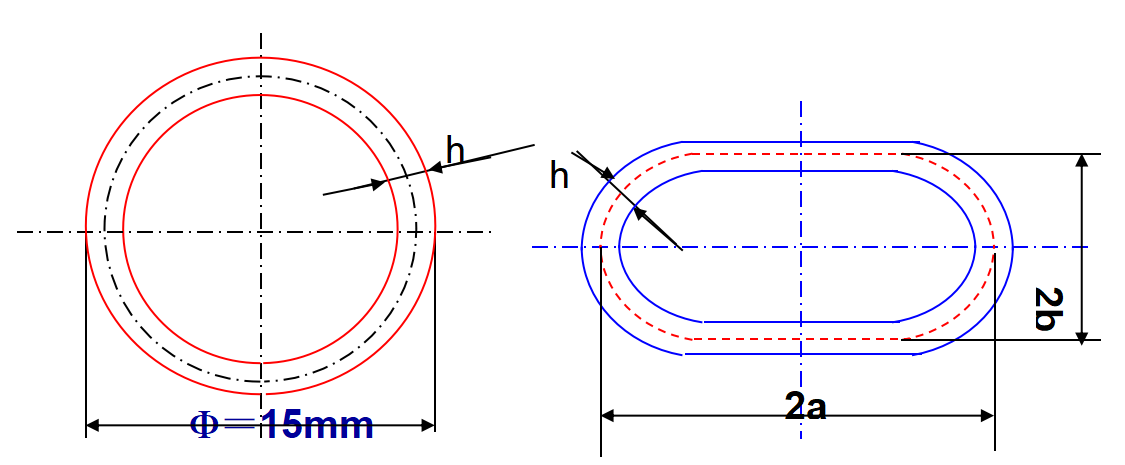
\includegraphics[width =\textwidth]{figures/3.1.png}
    \caption{弹簧管尺寸示意图}
    \label{FIGURE3.1}
\end{figure}
\subsection{曲柄滑块机构}
\begin{tabular}{@{}>{\raggedright\arraybackslash}p{0.4\linewidth}>{\raggedright\arraybackslash}p{0.4\linewidth}@{}}
相对杆长 : $\lambda=4$ &相对轴偏量 : $\varepsilon=1$\\
转动范围角 : $\alpha_p=50^\circ$ &初始位置角:$\alpha_0=-25^\circ$\\
终止位置角 : $\alpha_k=25^\circ$ &
\end{tabular}
\subsection{齿轮传动参数的选择}
\begin{tabular}{@{}>{\raggedright\arraybackslash}p{0.4\linewidth}>{\raggedright\arraybackslash}p{0.4\linewidth}@{}}
模数 : $m=0.7$ &传动比 : $i_{21}=5.4$\\
\end{tabular}
\subsection{标尺指针参数选择}
\begin{tabular}{@{}>{\raggedright\arraybackslash}p{0.4\linewidth}>{\raggedright\arraybackslash}p{0.4\linewidth}@{}}
分度尺寸:$6.75^{\circ}$ & 短标线长度:2mm\\
长标线长度:4mm & 指针与短标线重合长度:2mm\\
指针形状:楔杆形& 指针末端宽度:0.5mm
\end{tabular}
\subsection{游丝的选择}
\begin{tabular}{@{}>{\raggedright\arraybackslash}p{0.4\linewidth}>{\raggedright\arraybackslash}p{0.4\linewidth}@{}}
外径:$D_1=35mm$ & 内径:$D_2=6mm$\\
圈数:$n=9$ & 最小工作角度:$\phi_{min}={\pi}/{2}$\\
宽厚比:$\eta=6$ & 最大工作角度:$\phi_{max}=2{\pi}$\\
当量摩擦系数:$f_v=0.314$ & 摩擦系数:$f=0.2$
\end{tabular}